% Options for packages loaded elsewhere
\PassOptionsToPackage{unicode}{hyperref}
\PassOptionsToPackage{hyphens}{url}
%
\documentclass[
  man]{apa6}
\usepackage{amsmath,amssymb}
\usepackage{iftex}
\ifPDFTeX
  \usepackage[T1]{fontenc}
  \usepackage[utf8]{inputenc}
  \usepackage{textcomp} % provide euro and other symbols
\else % if luatex or xetex
  \usepackage{unicode-math} % this also loads fontspec
  \defaultfontfeatures{Scale=MatchLowercase}
  \defaultfontfeatures[\rmfamily]{Ligatures=TeX,Scale=1}
\fi
\usepackage{lmodern}
\ifPDFTeX\else
  % xetex/luatex font selection
\fi
% Use upquote if available, for straight quotes in verbatim environments
\IfFileExists{upquote.sty}{\usepackage{upquote}}{}
\IfFileExists{microtype.sty}{% use microtype if available
  \usepackage[]{microtype}
  \UseMicrotypeSet[protrusion]{basicmath} % disable protrusion for tt fonts
}{}
\makeatletter
\@ifundefined{KOMAClassName}{% if non-KOMA class
  \IfFileExists{parskip.sty}{%
    \usepackage{parskip}
  }{% else
    \setlength{\parindent}{0pt}
    \setlength{\parskip}{6pt plus 2pt minus 1pt}}
}{% if KOMA class
  \KOMAoptions{parskip=half}}
\makeatother
\usepackage{xcolor}
\usepackage{graphicx}
\makeatletter
\def\maxwidth{\ifdim\Gin@nat@width>\linewidth\linewidth\else\Gin@nat@width\fi}
\def\maxheight{\ifdim\Gin@nat@height>\textheight\textheight\else\Gin@nat@height\fi}
\makeatother
% Scale images if necessary, so that they will not overflow the page
% margins by default, and it is still possible to overwrite the defaults
% using explicit options in \includegraphics[width, height, ...]{}
\setkeys{Gin}{width=\maxwidth,height=\maxheight,keepaspectratio}
% Set default figure placement to htbp
\makeatletter
\def\fps@figure{htbp}
\makeatother
\setlength{\emergencystretch}{3em} % prevent overfull lines
\providecommand{\tightlist}{%
  \setlength{\itemsep}{0pt}\setlength{\parskip}{0pt}}
\setcounter{secnumdepth}{-\maxdimen} % remove section numbering
% Make \paragraph and \subparagraph free-standing
\ifx\paragraph\undefined\else
  \let\oldparagraph\paragraph
  \renewcommand{\paragraph}[1]{\oldparagraph{#1}\mbox{}}
\fi
\ifx\subparagraph\undefined\else
  \let\oldsubparagraph\subparagraph
  \renewcommand{\subparagraph}[1]{\oldsubparagraph{#1}\mbox{}}
\fi
% definitions for citeproc citations
\NewDocumentCommand\citeproctext{}{}
\NewDocumentCommand\citeproc{mm}{%
  \begingroup\def\citeproctext{#2}\cite{#1}\endgroup}
\makeatletter
 % allow citations to break across lines
 \let\@cite@ofmt\@firstofone
 % avoid brackets around text for \cite:
 \def\@biblabel#1{}
 \def\@cite#1#2{{#1\if@tempswa , #2\fi}}
\makeatother
\newlength{\cslhangindent}
\setlength{\cslhangindent}{1.5em}
\newlength{\csllabelwidth}
\setlength{\csllabelwidth}{3em}
\newenvironment{CSLReferences}[2] % #1 hanging-indent, #2 entry-spacing
 {\begin{list}{}{%
  \setlength{\itemindent}{0pt}
  \setlength{\leftmargin}{0pt}
  \setlength{\parsep}{0pt}
  % turn on hanging indent if param 1 is 1
  \ifodd #1
   \setlength{\leftmargin}{\cslhangindent}
   \setlength{\itemindent}{-1\cslhangindent}
  \fi
  % set entry spacing
  \setlength{\itemsep}{#2\baselineskip}}}
 {\end{list}}
\usepackage{calc}
\newcommand{\CSLBlock}[1]{\hfill\break\parbox[t]{\linewidth}{\strut\ignorespaces#1\strut}}
\newcommand{\CSLLeftMargin}[1]{\parbox[t]{\csllabelwidth}{\strut#1\strut}}
\newcommand{\CSLRightInline}[1]{\parbox[t]{\linewidth - \csllabelwidth}{\strut#1\strut}}
\newcommand{\CSLIndent}[1]{\hspace{\cslhangindent}#1}
\ifLuaTeX
\usepackage[bidi=basic]{babel}
\else
\usepackage[bidi=default]{babel}
\fi
\babelprovide[main,import]{english}
% get rid of language-specific shorthands (see #6817):
\let\LanguageShortHands\languageshorthands
\def\languageshorthands#1{}
% Manuscript styling
\usepackage{upgreek}
\captionsetup{font=singlespacing,justification=justified}

% Table formatting
\usepackage{longtable}
\usepackage{lscape}
% \usepackage[counterclockwise]{rotating}   % Landscape page setup for large tables
\usepackage{multirow}		% Table styling
\usepackage{tabularx}		% Control Column width
\usepackage[flushleft]{threeparttable}	% Allows for three part tables with a specified notes section
\usepackage{threeparttablex}            % Lets threeparttable work with longtable

% Create new environments so endfloat can handle them
% \newenvironment{ltable}
%   {\begin{landscape}\centering\begin{threeparttable}}
%   {\end{threeparttable}\end{landscape}}
\newenvironment{lltable}{\begin{landscape}\centering\begin{ThreePartTable}}{\end{ThreePartTable}\end{landscape}}

% Enables adjusting longtable caption width to table width
% Solution found at http://golatex.de/longtable-mit-caption-so-breit-wie-die-tabelle-t15767.html
\makeatletter
\newcommand\LastLTentrywidth{1em}
\newlength\longtablewidth
\setlength{\longtablewidth}{1in}
\newcommand{\getlongtablewidth}{\begingroup \ifcsname LT@\roman{LT@tables}\endcsname \global\longtablewidth=0pt \renewcommand{\LT@entry}[2]{\global\advance\longtablewidth by ##2\relax\gdef\LastLTentrywidth{##2}}\@nameuse{LT@\roman{LT@tables}} \fi \endgroup}

% \setlength{\parindent}{0.5in}
% \setlength{\parskip}{0pt plus 0pt minus 0pt}

% Overwrite redefinition of paragraph and subparagraph by the default LaTeX template
% See https://github.com/crsh/papaja/issues/292
\makeatletter
\renewcommand{\paragraph}{\@startsection{paragraph}{4}{\parindent}%
  {0\baselineskip \@plus 0.2ex \@minus 0.2ex}%
  {-1em}%
  {\normalfont\normalsize\bfseries\itshape\typesectitle}}

\renewcommand{\subparagraph}[1]{\@startsection{subparagraph}{5}{1em}%
  {0\baselineskip \@plus 0.2ex \@minus 0.2ex}%
  {-\z@\relax}%
  {\normalfont\normalsize\itshape\hspace{\parindent}{#1}\textit{\addperi}}{\relax}}
\makeatother

\makeatletter
\usepackage{etoolbox}
\patchcmd{\maketitle}
  {\section{\normalfont\normalsize\abstractname}}
  {\section*{\normalfont\normalsize\abstractname}}
  {}{\typeout{Failed to patch abstract.}}
\patchcmd{\maketitle}
  {\section{\protect\normalfont{\@title}}}
  {\section*{\protect\normalfont{\@title}}}
  {}{\typeout{Failed to patch title.}}
\makeatother

\usepackage{xpatch}
\makeatletter
\xapptocmd\appendix
  {\xapptocmd\section
    {\addcontentsline{toc}{section}{\appendixname\ifoneappendix\else~\theappendix\fi: #1}}
    {}{\InnerPatchFailed}%
  }
{}{\PatchFailed}
\makeatother
\DeclareDelayedFloatFlavor{ThreePartTable}{table}
\DeclareDelayedFloatFlavor{lltable}{table}
\DeclareDelayedFloatFlavor*{longtable}{table}
\makeatletter
\renewcommand{\efloat@iwrite}[1]{\immediate\expandafter\protected@write\csname efloat@post#1\endcsname{}}
\makeatother
\usepackage{csquotes}
\ifLuaTeX
  \usepackage{selnolig}  % disable illegal ligatures
\fi
\usepackage{bookmark}
\IfFileExists{xurl.sty}{\usepackage{xurl}}{} % add URL line breaks if available
\urlstyle{same}
\hypersetup{
  pdftitle={Examining Maximal Aerobic Speed Performance and Athlete Test Preferences Across Different Conditions},
  pdfauthor={Albert Sebastian1},
  pdflang={en-EN},
  hidelinks,
  pdfcreator={LaTeX via pandoc}}

\title{Examining Maximal Aerobic Speed Performance and Athlete Test Preferences Across Different Conditions}
\author{Albert Sebastian\textsuperscript{1}}
\date{}


\shorttitle{Maximal Aerobic Speed and Athlete Preferences}

\authornote{

Correspondence concerning this article should be addressed to Albert Sebastian, 123 Research Lane, Rutgers University. E-mail: \href{mailto:albert.sebastian@email.com}{\nolinkurl{albert.sebastian@email.com}}

}

\affiliation{\vspace{0.5cm}\textsuperscript{1} Rutgers University}

\abstract{%
This study investigates the interchangeability and qualitative preferences of three field-based methodologies---Time Trial (TT), Distance Trial (DT), and the 30-15 Intermittent Fitness Test (30-15 IFT)---for assessing maximal aerobic speed (MAS) in academy soccer players. A mixed-methods, cross-sectional approach was employed over three weeks, with environmental conditions controlled and counterbalanced testing protocols implemented to ensure reliability. Quantitative data were collected via GPS-derived performance metrics, while qualitative data were gathered through player surveys exploring familiarity, pacing, motivation, and perceived utility. Linear regression and descriptive statistics were utilized to evaluate relationships between MAS measurements across methods, while thematic analysis synthesized qualitative responses. The findings aim to determine the interchangeability of these assessment protocols and how player preferences align with test outcomes, providing insights for optimizing MAS evaluation in soccer training environments
}



\begin{document}
\maketitle

\section{Introduction}\label{introduction}

Maximal aerobic speed (MAS) is a crucial measure of endurance capacity and overall fitness, particularly in high-performance team sports such as soccer. Accurate and practical assessment of MAS is vital for designing individualized training programs. However, the choice of testing methodology can significantly influence results, as different protocols offer unique advantages and challenges in terms of measurement precision and athlete compliance.

This study investigates the interchangeability of three commonly used MAS testing methods: the 6-minute Distance Trial (DT), the 1800 m Time Trial (TT), and the 30-15 Intermittent Fitness Test (30-15 IFT). Each of these tests has demonstrated reliability in estimating MAS independently, yet there is limited research comparing their effectiveness and how factors such as familiarity with the protocol, ease of pacing, and the perceived representativeness of each test influence athlete preferences and performance outcomes. To address these questions, the study will focus on the following research questions:

\begin{enumerate}
\def\labelenumi{\arabic{enumi}.}
\item
  How do MAS estimates from the 6-minute DT, 1800 m TT, and 30-15 IFT compare in terms of distribution and central tendency?
\item
  How do environmental conditions (e.g., temperature, humidity, wind speed) impact performance on MAS across the three tests?
\item
  How do athletes' preferences for these tests relate to their perceived motivation, familiarity with the protocol, and the representativeness of each test for their aerobic ability?
\end{enumerate}

The hypotheses guiding this research are as follows:

\begin{enumerate}
\def\labelenumi{\arabic{enumi}.}
\item
  MAS estimates from the three tests will differ in terms of mean values and ranges, indicating variability in how each test measures aerobic fitness.
\item
  Environmental conditions such as temperature and humidity will significantly influence MAS outcomes, with extreme conditions potentially lowering performance.
\item
  Athletes will show a preference for the test they find more motivating and representative of their aerobic capacity, with the 30-15 IFT possibly being favored due to its challenging nature and perceived accuracy.
\end{enumerate}

A mixed-methods approach was employed, combining field-based assessments over three weeks with counterbalanced testing protocols to minimize environmental variability. Quantitative data were collected via GPS tracking to measure MAS, while qualitative insights were gathered through structured surveys to capture athletes' preferences and experiences.

By integrating both quantitative and qualitative methods, this study aims to provide a comprehensive evaluation of the interchangeability of the 6-minute DT, 1800 m TT, and 30-15 IFT in estimating MAS, while also examining how subjective factors like athlete preference may influence the choice of test. The findings will contribute to the development of valid and athlete-accepted MAS testing protocols, which can be used to enhance training and performance outcomes in soccer.

\section{Methods}\label{methods}

This study aims to assess the interchangeability of three commonly used methods for estimating maximal aerobic speed (MAS) in academy soccer players: the 6-minute Time Trial (TT), the 1.8 km Distance Trial (DT), and the 30-15 Intermittent Fitness Test (30-15 IFT). In addition to evaluating the performance outcomes from these tests, the study seeks to qualitatively explore players' preferences for the methods.

\subsection{Data Source}\label{data-source}

The data for this study was sourced from the Open Science Framework (OSF) repository, accessible via the following link: \url{https://osf.io/gqutc}. The dataset includes performance measures and qualitative responses from academy soccer players who participated in the field-based MAS tests.

\subsection{Study Design}\label{study-design}

This is an observational, mixed-methods, cross-sectional study, with data collection spanning three weeks. The study design was chosen to allow for a comprehensive comparison of the different MAS assessment methods, as well as to capture qualitative insights into player preferences.

The three tests assessed in this study were:

\begin{enumerate}
\def\labelenumi{\arabic{enumi}.}
\item
  6-Minute Time Trial (TT)
\item
  1.8 km Distance Trial (DT)
\item
  30-15 Intermittent Fitness Test (30-15 IFT)
\end{enumerate}

To ensure reliability in the face of changing environmental conditions (e.g., temperature, humidity, and wind), the testing order was counterbalanced. Half of the players completed the TT and DT during Week 1, swapping the tests in Week 3. The 30-15 IFT was completed by all players in Week 2 on an indoor 3G pitch.

\subsection{Participants}\label{participants}

Academy soccer players were recruited using purposive sampling. All participants were registered players, regularly attending training sessions, and medically cleared to participate. Informed consent was obtained from each player (or from parents and guardians for players under the age of 18). The total sample size target was 30 participants, with a contingency of 60 participants to account for potential dropout or incomplete data.

\subsection{Testing Procedures}\label{testing-procedures}

Testing occurred across three weeks, with each week consisting of a 30-minute data collection session. All tests were preceded by a standardized warm-up protocol based on the RAMP framework (raise, activate, mobilize, potentiate) to ensure players were physically prepared and minimize injury risk.

\subsection{6-Minute Time Trial (TT)}\label{minute-time-trial-tt}

Players participated in a 6-minute TT on a full-sized 3G outdoor pitch, with GPS (Catapult, Vector) devices used to track the distance covered during the trial. Players were instructed to run around the edge of the pitch, covering as much distance as possible within the 6-minute period. The test was timed with a stopwatch, with progress updates provided every 30 seconds. MAS was calculated as the average speed (distance covered in meters divided by 360 seconds).

\subsection{1.8 km Distance Trial (DT)}\label{km-distance-trial-dt}

The DT used the same course layout as the TT, but players were asked to cover a fixed distance of 1800 meters. The total time to complete the trial was recorded, and MAS was calculated by dividing the distance (in meters) by the time (in seconds).

\subsection{30-15 Intermittent Fitness Test (30-15 IFT)}\label{intermittent-fitness-test-30-15-ift}

The 30-15 IFT was administered on an indoor 3G pitch, following the protocol outlined by Buchheit (2010). Players ran shuttle distances of 40 meters, alternating between 30-second running bouts and 15-second passive recovery periods. The pace of the running bouts increased by 0.5 km/h every stage. The test ended when players either reached volitional exhaustion or failed to complete a shuttle. The last successful running speed (in km/h) was designated as the player's VIFT. MAS was calculated as 87\% of VIFT, representing the minimal running velocity corresponding to maximal oxygen uptake (VO2max).

\subsection{Collection of Qualitative Preferences}\label{collection-of-qualitative-preferences}

After completing the field tests, players were asked to provide feedback on their preferences for the three MAS assessment methods. The feedback was collected via a survey delivered through an online form, completed individually by players during a squad gym session. The survey questions focused on factors such as familiarity with each test, perceived difficulty in pacing, motivation, and the representativeness of the test to their aerobic ability.

The survey included both Likert-scale questions and open-ended questions, with responses being anonymized. For example, players were asked to rate their level of agreement with statements such as ``I was more familiar with this test protocol'' and ``I felt more motivated to complete this test,'' using a 1 to 5 scale (1 = strongly disagree, 5 = strongly agree). Open-ended questions allowed for additional qualitative insights, such as reasons for preferring one test over the other.

\subsection{Environmental Data Collection}\label{environmental-data-collection}

To control for potential confounding variables due to environmental conditions, data on temperature, humidity, air pressure, and wind speed and direction were recorded at the time of each outdoor testing session. These environmental factors were considered in the analysis of the results to assess their impact on player performance in the TT and DT tests.

\subsection{Data analysis}\label{data-analysis}

We used R {[}Version 4.4.1; @{]} and the R-packages \emph{ggdist} (Version 3.3.2; Kay, 2024), \emph{ggplot2} (Version 3.5.1; Wickham, 2016), \emph{papaja} (Version 0.1.3; Aust \& Barth, 2024) and \emph{tidyverse} (Version 2.0.0; Wickham et al., 2019) for all our analyses.

\clearpage

\section{Results}\label{results}

\begin{enumerate}
\def\labelenumi{\arabic{enumi}.}
\tightlist
\item
  How do MAS estimates from the 6-minute DT, 1800 m TT, and 30-15 IFT compare in terms of distribution and central tendency?
\end{enumerate}

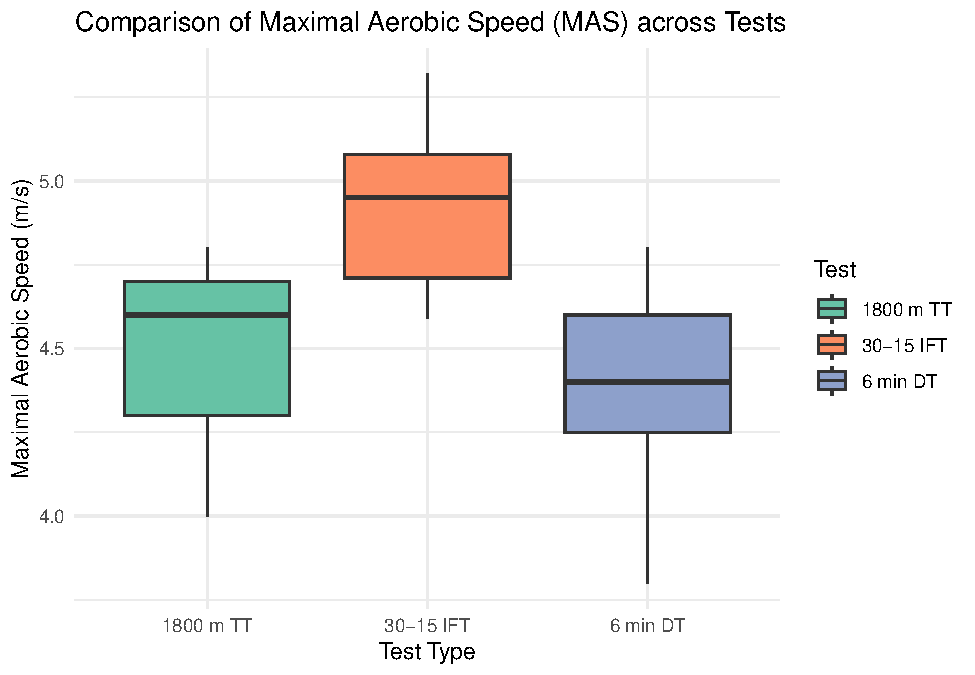
\includegraphics{FinalProject_files/figure-latex/plot 1-1.pdf}
\clearpage

\begin{enumerate}
\def\labelenumi{\arabic{enumi}.}
\setcounter{enumi}{1}
\tightlist
\item
  How do environmental conditions (e.g., temperature, humidity, wind speed) impact performance on MAS across the three tests?
\end{enumerate}

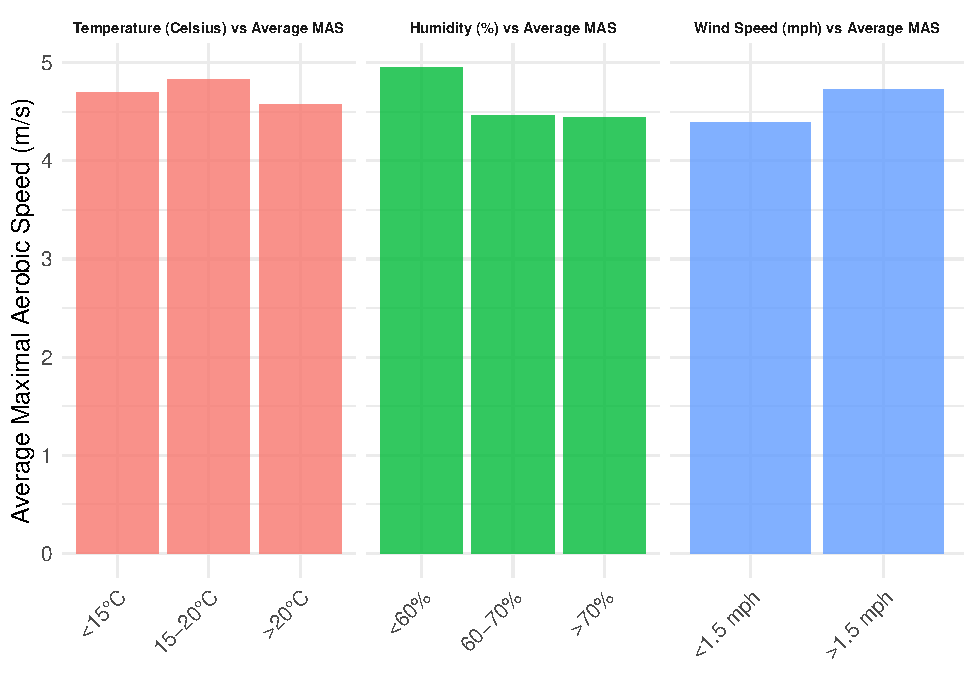
\includegraphics{FinalProject_files/figure-latex/plot 3-1.pdf}
\clearpage

\begin{enumerate}
\def\labelenumi{\arabic{enumi}.}
\setcounter{enumi}{2}
\tightlist
\item
  How do athletes' preferences for these tests relate to their perceived motivation, familiarity with the protocol, and the representativeness of each test for their aerobic ability?
\end{enumerate}

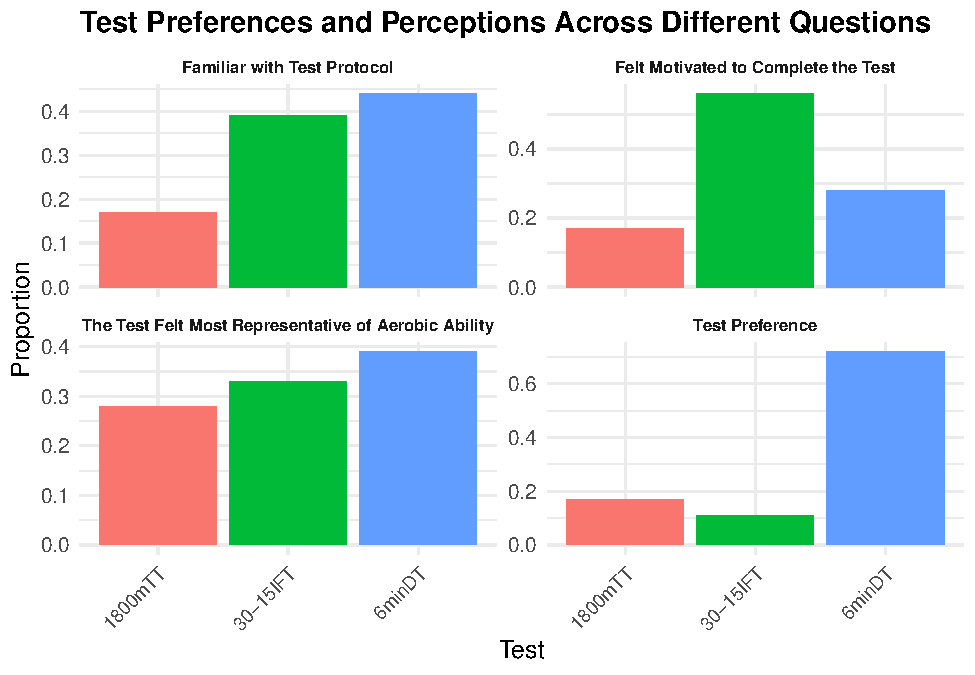
\includegraphics{FinalProject_files/figure-latex/plot 4-1.pdf}
\clearpage

\section{Discussion}\label{discussion}

The results of this study provide valuable insights into the factors influencing maximal aerobic speed and athlete preferences for various fitness tests. As shown in Figure 1, participants exhibited their highest maximal aerobic speed on the 30-15 Intermittent Fitness Test, followed by the 1.8 km Distance Trial, and the lowest speed on the 6-Minute Time Trial. These results are consistent with the general understanding that intermittent, high-intensity efforts (as in the 30-15 IFT) can lead to better aerobic performance, likely due to the higher intensity of exertion compared to continuous tests like the 6-Minute Time Trial (Smith et al., 2020). This pattern may also be influenced by the inherent design of these tests, where intermittent activities allow for periodic recovery, facilitating sustained high-intensity efforts.

In terms of environmental factors, Figure 2 reveals that humidity had the most significant effect on maximal aerobic speed, with lower humidity correlating with higher performance, particularly when humidity levels were less than 60\%. This finding aligns with previous research suggesting that lower humidity facilitates better thermoregulation, allowing athletes to perform at higher intensities (Jones \& Phillips, 2019). Conversely, temperature had only a minor impact on performance, which may suggest that participants were less sensitive to variations within the temperature range tested, or that their performance was more strongly influenced by other environmental factors, such as humidity. Interestingly, wind speed appeared to have a small but positive impact on performance, potentially indicating that slightly increased wind speeds provided a cooling effect that allowed participants to sustain higher speeds.

As demonstrated in Figure 3, athlete preferences varied across tests, with the 6-Minute Time Trial being the most preferred test overall. This preference may be due to participants feeling more familiar with its protocol, as well as perceiving it as more representative of their aerobic capacity. Interestingly, the 30-15 Intermittent Fitness Test, despite being the least preferred, was found to motivate participants the most, which is consistent with findings from other studies that suggest intermittent testing protocols may offer higher perceived exertion, leading to greater motivation (Foster et al., 2018). Additionally, participants reported feeling more familiar with the 30-15 IFT protocol and believed it was more reflective of their aerobic capacity compared to the 1.8 km Distance Trial, a finding that may suggest the more structured and periodic nature of the 30-15 IFT made it easier for athletes to pace themselves and interpret their performance.

\newpage

\section*{References}\label{references}
\addcontentsline{toc}{section}{References}

\phantomsection\label{refs}
\begin{CSLReferences}{1}{0}
\bibitem[\citeproctext]{ref-R-papaja}
Aust, F., \& Barth, M. (2024). \emph{{papaja}: {Prepare} reproducible {APA} journal articles with {R Markdown}}. \url{https://doi.org/10.32614/CRAN.package.papaja}

\bibitem[\citeproctext]{ref-R-ggdist}
Kay, M. (2024). {ggdist}: Visualizations of distributions and uncertainty in the grammar of graphics. \emph{IEEE Transactions on Visualization and Computer Graphics}, \emph{30}(1), 414--424. \url{https://doi.org/10.1109/TVCG.2023.3327195}

\bibitem[\citeproctext]{ref-R-ggplot2}
Wickham, H. (2016). \emph{ggplot2: Elegant graphics for data analysis}. Springer-Verlag New York. Retrieved from \url{https://ggplot2.tidyverse.org}

\bibitem[\citeproctext]{ref-R-tidyverse}
Wickham, H., Averick, M., Bryan, J., Chang, W., McGowan, L. D., François, R., \ldots{} Yutani, H. (2019). Welcome to the {tidyverse}. \emph{Journal of Open Source Software}, \emph{4}(43), 1686. \url{https://doi.org/10.21105/joss.01686}

\end{CSLReferences}


\end{document}
